\documentclass[12pt, a4paper, oneside]{article}\usepackage[]{graphicx}\usepackage[]{color}
%% maxwidth is the original width if it is less than linewidth
%% otherwise use linewidth (to make sure the graphics do not exceed the margin)
\makeatletter
\def\maxwidth{ %
  \ifdim\Gin@nat@width>\linewidth
    \linewidth
  \else
    \Gin@nat@width
  \fi
}
\makeatother

\definecolor{fgcolor}{rgb}{0.345, 0.345, 0.345}
\newcommand{\hlnum}[1]{\textcolor[rgb]{0.686,0.059,0.569}{#1}}%
\newcommand{\hlstr}[1]{\textcolor[rgb]{0.192,0.494,0.8}{#1}}%
\newcommand{\hlcom}[1]{\textcolor[rgb]{0.678,0.584,0.686}{\textit{#1}}}%
\newcommand{\hlopt}[1]{\textcolor[rgb]{0,0,0}{#1}}%
\newcommand{\hlstd}[1]{\textcolor[rgb]{0.345,0.345,0.345}{#1}}%
\newcommand{\hlkwa}[1]{\textcolor[rgb]{0.161,0.373,0.58}{\textbf{#1}}}%
\newcommand{\hlkwb}[1]{\textcolor[rgb]{0.69,0.353,0.396}{#1}}%
\newcommand{\hlkwc}[1]{\textcolor[rgb]{0.333,0.667,0.333}{#1}}%
\newcommand{\hlkwd}[1]{\textcolor[rgb]{0.737,0.353,0.396}{\textbf{#1}}}%

\usepackage{framed}
\makeatletter
\newenvironment{kframe}{%
 \def\at@end@of@kframe{}%
 \ifinner\ifhmode%
  \def\at@end@of@kframe{\end{minipage}}%
  \begin{minipage}{\columnwidth}%
 \fi\fi%
 \def\FrameCommand##1{\hskip\@totalleftmargin \hskip-\fboxsep
 \colorbox{shadecolor}{##1}\hskip-\fboxsep
     % There is no \\@totalrightmargin, so:
     \hskip-\linewidth \hskip-\@totalleftmargin \hskip\columnwidth}%
 \MakeFramed {\advance\hsize-\width
   \@totalleftmargin\z@ \linewidth\hsize
   \@setminipage}}%
 {\par\unskip\endMakeFramed%
 \at@end@of@kframe}
\makeatother

\definecolor{shadecolor}{rgb}{.97, .97, .97}
\definecolor{messagecolor}{rgb}{0, 0, 0}
\definecolor{warningcolor}{rgb}{1, 0, 1}
\definecolor{errorcolor}{rgb}{1, 0, 0}
\newenvironment{knitrout}{}{} % an empty environment to be redefined in TeX

\usepackage{alltt} % Paper size, default font size and one-sided paper
%\graphicspath{{./Figures/}} % Specifies the directory where pictures are stored
%\usepackage[dcucite]{harvard}
\usepackage{rotating}
\usepackage{setspace}
\usepackage{pdflscape}
\usepackage[flushleft]{threeparttable}
\usepackage{multirow}
\usepackage[comma, sort&compress]{natbib}% Use the natbib reference package - read up on this to edit the reference style; if you want text (e.g. Smith et al., 2012) for the in-text references (instead of numbers), remove 'numbers' 
\usepackage{graphicx}
%\bibliographystyle{plainnat}
\bibliographystyle{agsm}
\usepackage[colorlinks = true, citecolor = blue, linkcolor = blue]{hyperref}
%\hypersetup{urlcolor=blue, colorlinks=true} % Colors hyperlinks in blue - change to black if annoying
%\renewcommand[\harvardurl]{URL: \url}
\IfFileExists{upquote.sty}{\usepackage{upquote}}{}
\begin{document}
\title{Questions on Production 1}
\author{Rob Hayward} 
\date{\today}
\maketitle

\begin{enumerate}
\item What is the characteristic of \emph{short run} production? 
\begin{itemize}
\item A.  The relationship between the industry and the final product. 
\item B.   That there is one fixed factor of production
\item C.   The planning horizon of the business
\item D.    The period during which the firm must report its profits. 
\end{itemize}

B. The short run has one fixed factor of production. 

\item The slope of any line between the origin and the total product curve is
\begin{itemize}
\item A The way to find the maximum product
\item B The average product
\item C The maximum marginal product
\item D Impossible to draw
\end{itemize}

B.  A line from the origin to the Total Physical Product curve will represent the Output divided by the number of variable units.  This is the average product. 


\item The marginal product of labour is 
\begin{itemize}
\item A Total output produced by labour
\item B The change in total output from a small change in labour
\item C Total output less the cost of inputs
\item D The total cost of labour divided by its output
\end{itemize}

B. 

\item Which of these describe the production function
\begin{itemize}
\item A It shows the technological relationship between inputs and outputs
\item B  It expresses the relationship between costs and revenues
\item C It identifies the characteristics of a particular technology
\item  D It helps firms to maximise profits
\end{itemize}

A and C.  It shows the relationship between inputs and outputs for a particular technology.  If the technolgoy is changed, there is a new Total Physical Product curve. 

\item Which of the following are examples of fixed costs
\begin{itemize}
\item A The electricity bill
\item B Wages
\item C Gym membership
\item D Petrol
\end{itemize}

Probably C and maybe B.  Some wages may be more variable than others. 

\item The realtionship between the marginal cost and diminishing returns is
\begin{itemize}
\item A Diminishing returns are at points beyond the minium marginal cost
\item B Diminishing returns equal the marginal cost
\item C We do not know the relationship between marginal cost and diminishing returns
\item D It depends on the shape of the average product curve
\end{itemize}

A. The lowest point on the marginal cost curve is the point at which the diminishing returns sets in.  While there are increasing returns, there is more output for a given increase in input; once diminising returns set in, the inputs are achieving increasingly less output. 

\item Marginal cost
\begin{itemize}
\item A Cuts the peak of the Total Physical Product Curve
\item B Is always upward sloping
\item C Is always downward sloping
\item D Cuts the minimum on the average cost curve
\end{itemize}

D.  This is always the relationship between marginal and average. 

\item Which of these show diminishing returns?
\begin{itemize} 
\item A Marginal Product that is increasing at a slower rate
\item B A narrowing in the gap between average product and marginal product
\item C The peak in average physical product
\item D Marginal Product that is falling
\end{itemize}

A. The slope of the total physical product curve is the marginal product.  This will get steeper and steeper and then the steepness will start to diminish.  As the steepness diminishes, the diminishing returns are setting in. 

\item Please fill in the gaps in the following table that outlines the Total 
Physical Product (TPP), Average Physical Product (APP) and Marginal Physical Product (MPP) of a short-run production function with different levels of labour input.   



\begin{tabular}{c | p{2cm}p{2cm}p{2cm}p{2cm}}
Labour Input & TPP & APP & MP \\
\hline
0 & 0 & 0 & \\
  & & & 5 \\
1 & 5  &5  & \\
  & & & 7  \\
2 & 12 & 6 & \\
  & & & 8 \\
3 & 20& 6.67& \\
  & & &  5\\
4 & 25 & 6.25 & \\
  & & & 3\\
5 & 28 & 5.6 & \\
  & & & 2 \\
6 & 30 & 5 & \\
  & & & 0  \\
7 & 30 & 4.29 & \\
  & & &  -2\\
8 & 28 &3.5 & \\
  & & & -3  \\
9 & 25 & 2.78& \\
  & & & -5 \\
10 &20 & 2& \\
\hline
\end{tabular}
\item When you have completed the table, please plot the TPP and APP functions on a graph.

\begin{knitrout}
\definecolor{shadecolor}{rgb}{0.969, 0.969, 0.969}\color{fgcolor}

{\centering 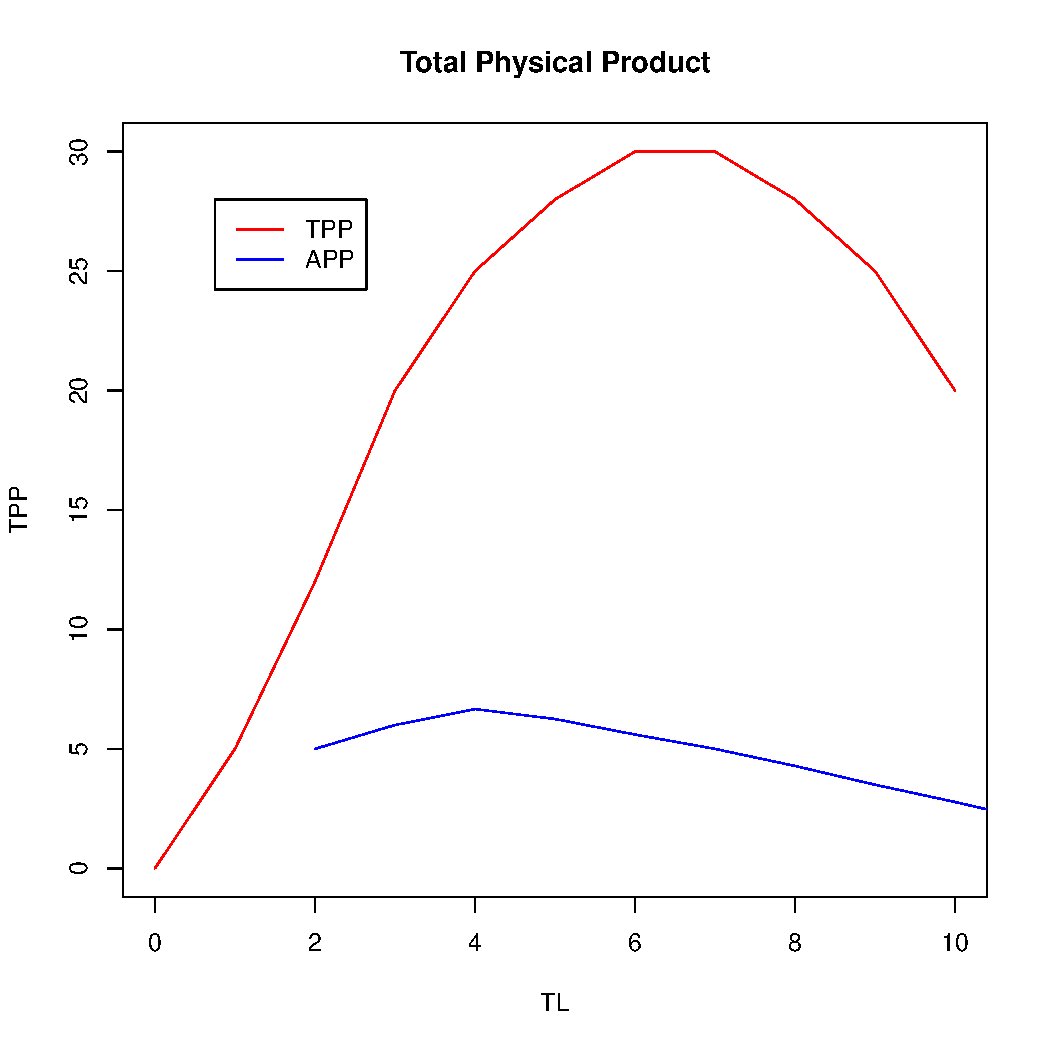
\includegraphics[width=\maxwidth]{figure/plot} 

}



\end{knitrout}


\item From the TPP curve, identify those points that represent the maximum and zero point of the MPP curve. 
\end{enumerate}
\end{document}
